\chapter{Gestione dei Requisiti}
\label{ch:GestioneDeiRequisiti}
\section{Requisiti Funzionali}
\label{sec:RequisitiFunzionali}

\newcounter{contrequisiti}\setcounter{contrequisiti}{1}

\paragraph{Area: Gestione Utenti}\mbox{}\\
% RF\thecontrequisiti: Persistenza informazioni\\
% Il sistema deve gestire l'archiviazione di dati su un supporto di memorizzazione non volatile.\vspace{10px} \\ \stepcounter{contrequisiti}
% RF\thecontrequisiti: Sicurezza Informazioni Personali\\
% Il sistema deve assicurare la tutela delle informazioni personali degli utenti\vspace{10px} \\ \stepcounter{contrequisiti}
% RF\thecontrequisiti: Gestisci Permessi\\
% Il sistema deve gestire i permessi ... .\vspace{10px} \\ \stepcounter{contrequisiti}
RF\thecontrequisiti: Crea Account Cliente\\
Il sistema dovrà permette al cliente di creare il proprio account.\vspace{10px} \\ \stepcounter{contrequisiti}
RF\thecontrequisiti: Aggiungi Dipendente\\
Il sistema dovrà permettere ad un impiegato già registrato di creare un account dipendente.\vspace{10px} \\ \stepcounter{contrequisiti}
RF\thecontrequisiti: Login Utente\\
Il sistema dovrà permettere all'utente di accedere al proprio account.\vspace{10px} \\ \stepcounter{contrequisiti}
RF\thecontrequisiti: Recupera Credenziali\\
Il sistema dovrà permettere all'utente di recuperare le credenziali del proprio account.\vspace{10px} \\ \stepcounter{contrequisiti}
RF\thecontrequisiti: Modifica Account\\
Il sistema dovrà permettere all'utente modificare le informazioni del proprio account.\vspace{10px} \\ \stepcounter{contrequisiti}

\paragraph{Area: Gestione Prodotto}\mbox{}\\
RF\thecontrequisiti: Aggiungi Prodotto al Catalogo\\
Il sistema dovrà permettere al dipendente di inserire un nuovo prodotto al catalogo.\vspace{10px} \\ \stepcounter{contrequisiti}
RF\thecontrequisiti: Modifica Prodotto del Catalogo\\
Il sistema dovrà permettere al dipendente di modificare un prodotto del catalogo.\vspace{10px} \\ \stepcounter{contrequisiti}
RF\thecontrequisiti: Rimuovi Prodotto dal Catalogo\\
Il sistema dovrà permettere al dipendente di rimuovere un prodotto dal catalogo.\vspace{10px} \\ \stepcounter{contrequisiti}
RF\thecontrequisiti: Aggiungi Categoria\\
Il sistema dovrà permettere al dipendente di inserire una nuova categoria di prodotti con la relativa immagine.\vspace{10px} \\ \stepcounter{contrequisiti}
RF\thecontrequisiti: Ordina Categorie\\
Il sistema dovrà permettere al dipendente di modificare l'ordine di visualizzazione delle categorie.\vspace{10px} \\ \stepcounter{contrequisiti}
RF\thecontrequisiti: Aggiungi Brand\\
Il sistema dovrà permettere al dipendente di inserire una nuovo brand di prodotti.\vspace{10px} \\ \stepcounter{contrequisiti}
RF\thecontrequisiti: Aggiungi Colore\\
Il sistema dovrà permettere al dipendente di inserire un nuovo colore.\vspace{10px} \\ \stepcounter{contrequisiti}
RF\thecontrequisiti: Aggiungi Taglia\\
Il sistema dovrà permettere al dipendente di inserire una nuova taglia.\vspace{10px} \\ \stepcounter{contrequisiti}
RF\thecontrequisiti: Ordina Taglie\\
Il sistema dovrà permettere al dipendente di modificare l'ordine di visualizzazione delle taglie.\vspace{10px} \\ \stepcounter{contrequisiti}


\paragraph{Area: Navigazione Prodotti}\mbox{}\\
RF\thecontrequisiti: Visualizza Prodotto\\
Il sistema dovrà mostrare le informazioni dettagliate di un prodotto.\vspace{10px} \\ \stepcounter{contrequisiti}
RF\thecontrequisiti: Visualizza Catalogo\\
Il sistema dovrà mostrare al cliente i prodotti presenti nel catalogo.\vspace{10px} \\ \stepcounter{contrequisiti}
RF\thecontrequisiti: Cerca Prodotto\\
Il sistema dovrà permettere al cliente di cercare il prodotto desiderato tramite ricerca testuale.\vspace{10px} \\ \stepcounter{contrequisiti}
RF\thecontrequisiti: Filtra Prodotti\\
Il sistema dovrà permettere al cliente di filtrare i prodotti tramite filtri per marca, colore e taglia.\vspace{10px} \\ \stepcounter{contrequisiti}


\paragraph{Area: Gestione Carrello}\mbox{}\\
RF\thecontrequisiti: Aggiungi Prodotto al Carrello\\
Il sistema dovrà permettere al cliente di inserire un prodotto nel carrello.\vspace{10px} \\ \stepcounter{contrequisiti}
RF\thecontrequisiti: Modifica Prodotto del Carrello\\
Il sistema dovrà permettere al cliente di modificare la quantità e lo stato di un prodotto nel carrello.\vspace{10px} \\ \stepcounter{contrequisiti}
RF\thecontrequisiti: Rimuovi Prodotto dal Carrello\\
Il sistema dovrà permettere al cliente di rimuovere un prodotto dal carrello.\vspace{10px} \\ \stepcounter{contrequisiti}
RF\thecontrequisiti: Visualizza Carrello\\
Il sistema dovrà permettere al cliente di visualizzare i prodotti nel carrello.\vspace{10px} \\ \stepcounter{contrequisiti}

\paragraph{Area: Gestione Ordine}\mbox{}\\
RF\thecontrequisiti: Effettua Ordine\\
Il sistema dovrà permettere al cliente di effettuare un ordine.\vspace{10px} \\ \stepcounter{contrequisiti}
RF\thecontrequisiti: Visualizza Ordine\\
Il sistema dovrà permettere al cliente di visualizzare i dettagli di un ordine effettuato.\vspace{10px} \\ \stepcounter{contrequisiti}
RF\thecontrequisiti: Visualizza Storico Ordini\\
Il sistema dovrà permettere al cliente di visualizzare i dettagli di un ordine effettuato.\vspace{10px} \\ \stepcounter{contrequisiti}
RF\thecontrequisiti: Richiedi Reso\\
Il sistema dovrà permettere al cliente di richiedere il reso di un prodotto.\vspace{10px} \\ \stepcounter{contrequisiti}


\paragraph{Area: Gestione Recensione}\mbox{}\\
RF\thecontrequisiti: Pubblica Recensione\\
Il sistema dovrà permettere al cliente di pubblicare recensioni per prodotti che ha acquistato.\vspace{10px} \\ \stepcounter{contrequisiti}
RF\thecontrequisiti: Modifica Recensione\\
Il sistema dovrà permettere al cliente di modificare le recensioni che ha precedentemente pubblicato.\vspace{10px} \\ \stepcounter{contrequisiti}
RF\thecontrequisiti: Elimina Recensione\\
Il sistema dovrà permettere al cliente di eliminare una recensione che ha precedentemente pubblicato.\vspace{10px} \\ \stepcounter{contrequisiti}


\setcounter{contrequisiti}{1}
\section{Requisiti non Funzionali}
\label{sec:RequisitiNonFunzionali}

\paragraph{Area: Gestione Tecnologie - vincoli}\mbox{}\\
RNF\thecontrequisiti: Implementazione in Python 3\\
Il sistema dovrà essere implementato in linguaggio Python 3.\vspace{10px} \\ \stepcounter{contrequisiti}
RNF\thecontrequisiti: Utilizzo di un Database relazionale\\
Il sistema dovrà adoperare un database relazionale per il salvataggio dei dati.\vspace{10px} \\ \stepcounter{contrequisiti}
RNF\thecontrequisiti: Verfica Email\\
Il sistema dovrà verificare, durante la registrazione, che l'utente è il proprietario dell'email inserita.\vspace{10px} \\ \stepcounter{contrequisiti}
RNF\thecontrequisiti: Gestione Recupero Credenziali tramite Email\\
Il sistema permetterà all'utente di recuperare le proprie credenziali tramite email.\vspace{10px} \\ \stepcounter{contrequisiti}
RNF\thecontrequisiti: Trasferimento Prodotti Carrello\\
Il sistema, al momento del login, trasferirà tutti i prodotti attualmente presenti nel carrello nel nuovo profilo.\vspace{10px} \\ \stepcounter{contrequisiti}
RNF\thecontrequisiti: Notifica Ordine Effettuato\\
Il sistema dovrà notificare il cliente quando viene effettuato un'ordine con successo.\vspace{10px} \\ \stepcounter{contrequisiti}


\newpage\section{Diagrammi dei casi d'uso}
\label{sec:DiagrammiDeiCasiDuso}

\newcounter{IDCasiDuso}\setcounter{IDCasiDuso}{1}
\paragraph{Diagramma Gestione Utente}\mbox{}\\
\begin{center}
  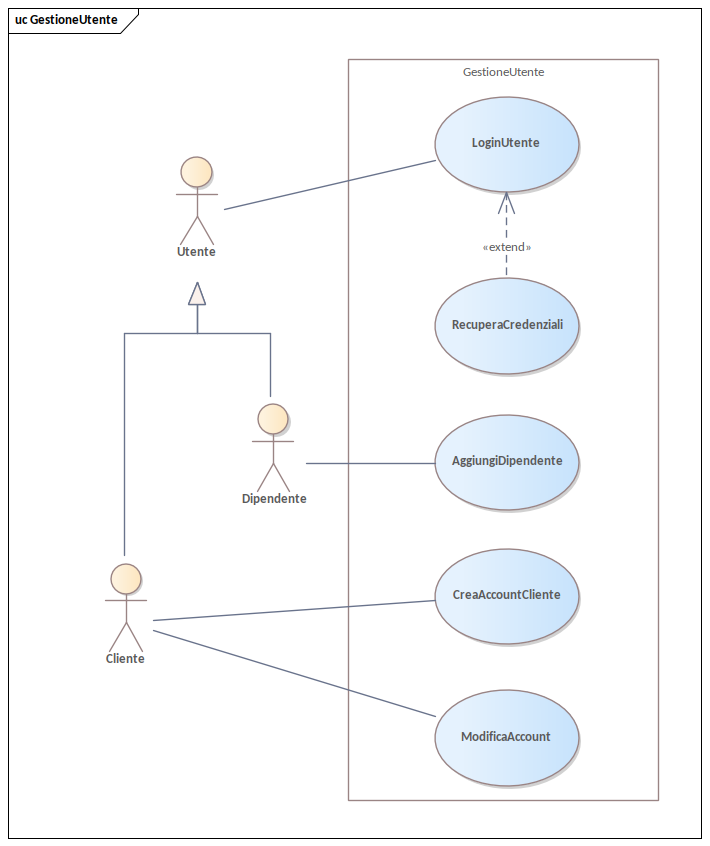
\includegraphics[width=\textwidth, height=20cm, keepaspectratio]{immagini/GestioneDeiRequisiti/GestioneUtente.png}
\end{center}

%%%%%%%% Copiato dai pdf di Ursino -  Gestione dei requisiti p.65 %%%%%%%%
\newpage
\paragraph{Caso d'uso: CreaAccountCliente}\mbox{}\\
\begin{center}
\begin{tabular}{ |p{12cm}| } 
    \hline
    \textbf{Caso d'uso: CreaAccountCliente} \\
    \hline
    \textbf{ID:} \theIDCasiDuso \stepcounter{IDCasiDuso} \\
    \hline
    \textbf{Breve Descrizione:} \\
    Il sistema crea un nuovo account per il Cliente. \\
    \hline
    \textbf{Attori Primari:} \\
    Cliente \\
    \hline
    \textbf{Attori Secondari:} \\
    Nessuno \\
    \hline
    \textbf{Precondizioni:} \\
    Nessuna \\
    \hline 
    \textbf{Sequenza degli eventi principale:}
    \begin{enumerate}[nosep, left=0pt]
        \item Il caso d'uso inizia quando il Cliente seleziona "Crea nuovo account".
        \item \textbf{While} le informazioni del Cliente non sono valide
    	\begin{enumerate}[nosep, left=0pt]
    		\item Il sistema chiede al Cliente di inserire le sue informazioni: nome, cognome, email, e password. 
    		\item Il sistema valida le informazioni del Cliente. 
        \end{enumerate} 
    \item Il sistema crea un nuovo account per il Cliente.
    \end{enumerate} \\
    \hline
    \textbf{Postcondizioni:}
	\begin{enumerate}[nosep, left=0pt]
    	\item Un nuovo account è stato creato per il Cliente. 
    \end{enumerate} \\
    \hline
    \textbf{Sequenza degli eventi alternativa:} \\
    Nessuna \\
    \hline
\end{tabular}
\end{center}

\newpage
\paragraph{Caso d'uso: AggiungiDipendente}\mbox{}\\
\begin{center}
\begin{tabular}{ |p{12cm}| } 
    \hline
    \textbf{Caso d'uso: AggiungiDipendente} \\
    \hline
    \textbf{ID:} \theIDCasiDuso \stepcounter{IDCasiDuso} \\
    \hline
    \textbf{Breve Descrizione:} \\
    Il sistema crea un account per il nuovo dipendente. \\
    \hline
    \textbf{Attori Primari:} \\
    Dipendente \\
    \hline
    \textbf{Attori Secondari:} \\
    Nessuno \\
    \hline
    \textbf{Precondizioni:} \\
    Nessuna \\
    \hline 
    \textbf{Sequenza degli eventi principale:}
    \begin{enumerate}[nosep, left=0pt]
        \item Il caso d'uso inizia quando un Dipendente seleziona "Aggiungi dipendente".
        \item \textbf{While} le informazioni del nuovo dipendente non sono valide
    	\begin{enumerate}[nosep, left=0pt]
    		\item Il Dipendente inserisce le informazioni del nuovo dipendente: nome, cognome, email. 
    		\item Il sistema valida le informazioni del nuovo dipendente. 
        \end{enumerate} 
        \item Il sistema genera una password per il nuovo dipendente.
        \item Il sistema crea un nuovo account per il nuovo dipendente.
        \item Il sistema invia la password al nuovo dipendente tramite il suo indirizzo di posta elettronica.
    \end{enumerate} \\
    \hline
    \textbf{Postcondizioni:}
	\begin{enumerate}[nosep, left=0pt]
    		\item Un nuovo account è stato creato per il nuovo dipendente. 
    	\end{enumerate} \\
    \hline
    \textbf{Sequenza degli eventi alternativa:} \\
    Nessuna \\
    \hline
\end{tabular}
\end{center}

\newpage\paragraph{Caso d'uso: LoginUtente}\mbox{}\\
\begin{center}
\begin{tabular}{ |p{12cm}| } 
    \hline
    \textbf{Caso d'uso: LoginUtente} \\
    \hline
    \textbf{ID:} \theIDCasiDuso \stepcounter{IDCasiDuso} \\
    \hline
    \textbf{Breve Descrizione:} \\
    Permette all'Utente di accedere al proprio account. \\
    \hline
    \textbf{Attori Primari:} \\
    Utente \\
    \hline
    \textbf{Attori Secondari:} \\
    Nessuno \\
    \hline
    \textbf{Precondizioni:}
    \begin{enumerate}[nosep, left=0pt]
        \item L'Utente deve essere già registrato.
    \end{enumerate} \\
    \hline
    \textbf{Sequenza degli eventi principale:}
    \begin{enumerate}[nosep, left=0pt]
        \item Il caso d'uso inizia quando l'Utente seleziona "Accedi".
        \item[]\hspace*{-0.65cm} punto di estensione: Recupera credenziali
        \item \textbf{While} le credenziali inserite dall'Utente non sono valide
    	\begin{enumerate}[nosep, left=0pt]
    		\item Il sistema chiede all'Utente di inserire email e password.
    		\item Il sistema valida le credenziali inserite dall'Utente. 
        \end{enumerate} 
        \item Il sistema autentica l'Utente.
    \end{enumerate} \\
    \hline
    \textbf{Postcondizioni:}
    \begin{enumerate}[nosep, left=0pt]
        \item L'Utente ha effettuato il login al proprio account.
    \end{enumerate} \\
    \hline
    \textbf{Sequenza degli eventi alternativa:} \\
    Nessuna \\
    \hline
\end{tabular}
\end{center}

\newpage\paragraph{Caso d'uso di estensione: RecuperaCredenziali}\mbox{}\\
\begin{center}
\begin{tabular}{ |p{12cm}| } 
    \hline
    \textbf{Caso d'uso di estensione: RecuperaCredenziali} \\
    \hline
    \textbf{ID:} \theIDCasiDuso \stepcounter{IDCasiDuso} \\
    \hline
    \textbf{Breve Descrizione:} \\
    Segmento 1: L'Utente recupera le credenziali del proprio account in caso di smarrimento della password. \\
    \hline
    \textbf{Attori Primari:} \\
    Utente \\
    \hline
    \textbf{Attori Secondari:} \\
    Nessuno \\
    \hline
    \textbf{Precondizioni del segmento 1:}
    \begin{enumerate}[nosep, left=0pt]
        \item L'Utente ha un account registrato nel sistema.
        \item L'Utente visualizza la schermata di login.
        \item L'Utente seleziona l'opzione "Recupera credenziali".
    \end{enumerate} \\
    \hline
    \textbf{Sequenza degli eventi del segmento 1:}
    \begin{enumerate}[nosep, left=0pt]
        \item \textbf{While} l'email inserita dall'Utente non è registrata
    	\begin{enumerate}[nosep, left=0pt]
    		\item Il sistema chiede all'Utente di inserire la sua email.
    		\item Il sistema valida l'email inserita dall'Utente. 
        \end{enumerate} 
        \item Il sistema genera una nuova password e la invia all'indirizzo email fornito.
        \item L'Utente riceve la mail e utilizza la nuova password per accedere al proprio account.
    \end{enumerate} \\
    \hline
    \textbf{Postcondizioni del segmento 1:}
    \begin{enumerate}[nosep, left=0pt]
        \item L'Utente può accedere al proprio account utilizzando la nuova password.
    \end{enumerate} \\
    \hline
\end{tabular}
\end{center}   

\newpage\paragraph{Caso d'uso: ModificaAccount}\mbox{}\\
\begin{center}
\begin{tabular}{ |p{12cm}| } 
    \hline
    \textbf{Caso d'uso: ModificaAccount} \\
    \hline
    \textbf{ID:} \theIDCasiDuso \stepcounter{IDCasiDuso} \\
    \hline
    \textbf{Breve Descrizione:} \\
    Permette al Cliente di modificare le informazioni del proprio account. \\
    \hline
    \textbf{Attori Primari:} \\
    Cliente \\
    \hline
    \textbf{Attori Secondari:} \\
    Nessuno \\
    \hline
    \textbf{Precondizioni:}
    \begin{enumerate}[nosep, left=0pt]
        \item Il Cliente deve essere registrato alla piattaforma.
        \item Il Cliente deve aver effettuato l'accesso al proprio account.
        \item Il Cliente deve visualizzare la pagina del profilo.
    \end{enumerate} \\
    \hline
    \textbf{Sequenza degli eventi principale:}
    \begin{enumerate}[nosep, left=0pt]
        \item Il caso d'uso inizia quando il Cliente seleziona "Modifica Account".
        \item \textbf{While} le credenziali inserite dal Cliente non sono valide:
    	\begin{enumerate}[nosep, left=0pt]
    		\item Il sistema chiede  al Cliente di inserire le nuove informazioni: nome, cognome e email.
                \item Il Cliente inserisce le informazioni richieste dal sistema.
    		\item Il sistema valida le credenziali inserite dal Cliente.
        \end{enumerate}
        \item Il sistema aggiorna le informazioni del profilo del Cliente.
    \end{enumerate} \\
    \hline
    \textbf{Postcondizioni:}
    \begin{enumerate}[nosep, left=0pt]
        \item Le informazioni dell'account del Cliente sono state aggiornate.
    \end{enumerate} \\
    \hline
    \textbf{Sequenza degli eventi alternativa:} \\
    Nessuna \\
    \hline
\end{tabular}
\end{center}


\newpage\paragraph{Diagramma Gestione Prodotto}\mbox{}\\
\begin{center}
  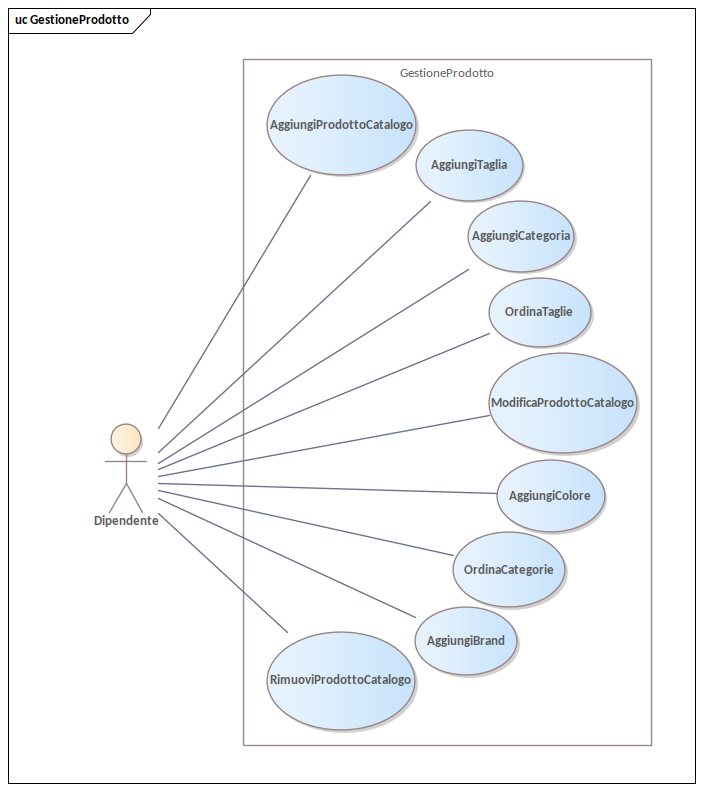
\includegraphics[width=\textwidth, height=20cm, keepaspectratio]{immagini/GestioneDeiRequisiti/GestioneProdotto.png}
\end{center}

\newpage
\paragraph{Caso d'uso: AggiungiProdottoCatalogo}\mbox{}\\
\begin{center}
\begin{tabular}{ |p{12cm}| } 
    \hline
    \textbf{Caso d'uso: AggiungiProdottoCatalogo} \\
    \hline
    \textbf{ID:} \theIDCasiDuso \stepcounter{IDCasiDuso} \\
    \hline
    \textbf{Breve Descrizione:} \\
    Un Dipendente aggiunge un prodotto al catalogo. \\
    \hline
    \textbf{Attori Primari:} \\
    Dipendente \\
    \hline
    \textbf{Attori Secondari:} \\
    Nessuno \\
    \hline
    \textbf{Precondizioni:} 
    \begin{enumerate}[nosep, left=0pt]
	    \item Il Dipendente ha effettuato il login al proprio account.
	    \item Il prodotto non è già presente nel catalogo.
    \end{enumerate} \\
    \hline 
    \textbf{Sequenza degli eventi principale:}
    \begin{enumerate}[nosep, left=0pt]
        \item Il caso d'uso inizia quando il dipendente seleziona "Aggiungi prodotto".
	    \item Il sistema richiede al Dipendente di inserire le seguenti informazioni del nuovo prodotto: titolo, descrizione, prezzo, colore, taglia, immagini per ciascuna alternativa di colore, quantità disponibile per ciascuna alternativa di colore e taglia.
        \item Il Dipendente inserisce le informazioni del prodotto richieste.
	    \item Il sistema aggiunge il prodotto al catalogo.
    \end{enumerate} \\
    \hline
    \textbf{Postcondizioni:}
	\begin{enumerate}[nosep, left=0pt]
    	\item Il prodotto è stato aggiunto al catalogo. 
		\item Il prodotto può essere visto dai visitatori del sito.
    \end{enumerate} \\
    \hline
    \textbf{Sequenza degli eventi alternativa:} \\
    Nessuna \\
    \hline
\end{tabular}
\end{center}

\newpage
\paragraph{Caso d'uso: ModificaProdottoCatalogo}\mbox{}\\
\begin{center}
\begin{tabular}{ |p{12cm}| } 
    \hline
    \textbf{Caso d'uso: ModificaProdottoCatalogo} \\
    \hline
    \textbf{ID:} \theIDCasiDuso \stepcounter{IDCasiDuso} \\
    \hline
    \textbf{Breve Descrizione:} \\
    Un Dipendente modifica le informazioni di un prodotto già presente nel catalogo. \\
    \hline
    \textbf{Attori Primari:} \\
    Dipendente \\
    \hline
    \textbf{Attori Secondari:} \\
    Nessuno \\
    \hline
    \textbf{Precondizioni:} 
    \begin{enumerate}[nosep, left=0pt]
	    \item Il Dipendente ha effettuato il login al proprio account.
	    \item Il prodotto è già presente nel catalogo.
    \end{enumerate} \\
    \hline 
    \textbf{Sequenza degli eventi principale:}
    \begin{enumerate}[nosep, left=0pt]
        \item Il caso d'uso inizia quando il dipendente seleziona "Modifica prodotto".
	    \item Il sistema mostra le informazioni correnti del prodotto selezionato.
        \item Il Dipendente modifica le informazioni del prodotto.
	    \item Il sistema aggiorna il prodotto.
    \end{enumerate} \\
    \hline
    \textbf{Postcondizioni:}
	\begin{enumerate}[nosep, left=0pt]
    	\item Le informazioni del prodotto sono state aggiornate.
		\item Le informazioni aggiornate del prodotto sono visibili ai clienti sulla piattaforma.
    \end{enumerate} \\
    \hline
    \textbf{Sequenza degli eventi alternativa:} \\
    Nessuna \\
    \hline
\end{tabular}
\end{center}

\newpage
\paragraph{Caso d'uso: RimuoviProdottoCatalogo}\mbox{}\\
\begin{center}
\begin{tabular}{ |p{12cm}| } 
    \hline
    \textbf{Caso d'uso: RimuoviProdottoCatalogo} \\
    \hline
    \textbf{ID:} \theIDCasiDuso \stepcounter{IDCasiDuso} \\
    \hline
    \textbf{Breve Descrizione:} \\
    Un Dipendente rimuove un prodotto dal catalogo. \\
    \hline
    \textbf{Attori Primari:} \\
    Dipendente \\
    \hline
    \textbf{Attori Secondari:} \\
    Nessuno \\
    \hline
    \textbf{Precondizioni:} 
    \begin{enumerate}[nosep, left=0pt]
	    \item Il Dipendente ha effettuato il login al proprio account.
	    \item Il prodotto è presente nel catalogo.
    \end{enumerate} \\
    \hline 
    \textbf{Sequenza degli eventi principale:}
    \begin{enumerate}[nosep, left=0pt]
        \item Il caso d'uso inizia quando il dipendente seleziona "Rimuovi prodotto".
	    \item Il sistema rimuove il prodotto dal catalogo.
    \end{enumerate} \\
    \hline
    \textbf{Postcondizioni:}
	\begin{enumerate}[nosep, left=0pt]
    	\item Il prodotto non è più disponibile per l'acquisto.
    \end{enumerate} \\
    \hline
    \textbf{Sequenza degli eventi alternativa:} \\
    Nessuna \\
    \hline
\end{tabular}
\end{center}

\newpage\paragraph{Caso d'uso: AggiungiCategoria}\mbox{}\\
\begin{center}
\begin{tabular}{ |p{12cm}| } 
    \hline
    \textbf{Caso d'uso: AggiungiCategoria} \\
    \hline
    \textbf{ID:} \theIDCasiDuso \stepcounter{IDCasiDuso} \\
    \hline
    \textbf{Breve Descrizione:} \\
    Un Dipendente aggiunge una nuova categoria. \\
    \hline
    \textbf{Attori Primari:} \\
    Dipendente \\
    \hline
    \textbf{Attori Secondari:} \\
    Nessuno \\
    \hline
    \textbf{Precondizioni:} 
    \begin{enumerate}[nosep, left=0pt]
	    \item Il Dipendente ha effettuato il login al proprio account.
	    \item La categoria non è già stata inserita.
    \end{enumerate} \\
    \hline 
    \textbf{Sequenza degli eventi principale:}
    \begin{enumerate}[nosep, left=0pt]
        \item Il caso d'uso inizia quando il dipendente seleziona "Aggiungi categoria".
	    \item Il sistema richiede al Dipendente di inserire le seguenti informazioni della nuova categoria: categoria padre, nome, posizione e immagine.
        \item Il Dipendente inserisce le informazioni della categoria richieste.
	    \item Il sistema aggiunge la nuova categoria.
    \end{enumerate} \\
    \hline
    \textbf{Postcondizioni:}
	\begin{enumerate}[nosep, left=0pt]
    	\item La categoria è stata aggiunta al sito.
        \item La categoria è selezionabile dall'utente nei filtri di ricerca.
    \end{enumerate} \\
    \hline
    \textbf{Sequenza degli eventi alternativa:} \\
    Nessuna \\
    \hline
\end{tabular}
\end{center}

\newpage\paragraph{Caso d'uso: OrdinaCategorie}\mbox{}\\
\begin{center}
\begin{tabular}{ |p{12cm}| } 
    \hline
    \textbf{Caso d'uso: OrdinaCategorie} \\
    \hline
    \textbf{ID:} \theIDCasiDuso \stepcounter{IDCasiDuso} \\
    \hline
    \textbf{Breve Descrizione:} \\
    Un Dipendente ordina le categorie esistenti. \\
    \hline
    \textbf{Attori Primari:} \\
    Dipendente \\
    \hline
    \textbf{Attori Secondari:} \\
    Nessuno \\
    \hline
    \textbf{Precondizioni:} 
    \begin{enumerate}[nosep, left=0pt]
	    \item Il Dipendente ha effettuato il login al proprio account.
	    \item La categoria è presente nel sito.
    \end{enumerate} \\
    \hline 
    \textbf{Sequenza degli eventi principale:}
    \begin{enumerate}[nosep, left=0pt]
        \item Il caso d'uso inizia quando il dipendente seleziona "Ordina categoria".
	    \item Il sistema richiede al Dipendente di inserire la nuova posizione della categoria nei confronti delle categorie con la stessa categoria padre.
        \item Il Dipendente inserisce la nuova posizione della categoria.
	    \item Il sistema modifica la posizione della categoria.
    \end{enumerate} \\
    \hline
    \textbf{Postcondizioni:}
	\begin{enumerate}[nosep, left=0pt]
    	\item La categoria viene visualizzata nella nuova posizione definita dal Dipendente.
    \end{enumerate} \\
    \hline
    \textbf{Sequenza degli eventi alternativa:} \\
    Nessuna \\
    \hline
\end{tabular}
\end{center}

\newpage\paragraph{Caso d'uso: AggiungiBrand}\mbox{}\\
\begin{center}
\begin{tabular}{ |p{12cm}| } 
    \hline
    \textbf{Caso d'uso: AggiungiBrand} \\
    \hline
    \textbf{ID:} \theIDCasiDuso \stepcounter{IDCasiDuso} \\
    \hline
    \textbf{Breve Descrizione:} \\
    Un Dipendente aggiunge un nuovo brand. \\
    \hline
    \textbf{Attori Primari:} \\
    Dipendente \\
    \hline
    \textbf{Attori Secondari:} \\
    Nessuno \\
    \hline
    \textbf{Precondizioni:} 
    \begin{enumerate}[nosep, left=0pt]
	    \item Il Dipendente ha effettuato il login al proprio account.
	    \item Il brand non è già stato inserito.
    \end{enumerate} \\
    \hline 
    \textbf{Sequenza degli eventi principale:}
    \begin{enumerate}[nosep, left=0pt]
        \item Il caso d'uso inizia quando il dipendente seleziona "Aggiungi brand".
	    \item Il sistema richiede al Dipendente di inserire le seguenti informazioni del nuovo brand: nome e immagine.
        \item Il Dipendente inserisce le informazioni del brand richieste.
	    \item Il sistema aggiunge il nuovo brand.
    \end{enumerate} \\
    \hline
    \textbf{Postcondizioni:}
	\begin{enumerate}[nosep, left=0pt]
    	\item Il brand è stato aggiunto al sito.
        \item Il brand è selezionabile dall'utente nei filtri di ricerca.
    \end{enumerate} \\
    \hline
    \textbf{Sequenza degli eventi alternativa:} \\
    Nessuna \\
    \hline
\end{tabular}
\end{center}

\newpage\paragraph{Caso d'uso: AggiungiColore}\mbox{}\\
\begin{center}
\begin{tabular}{ |p{12cm}| } 
    \hline
    \textbf{Caso d'uso: AggiungiColore} \\
    \hline
    \textbf{ID:} \theIDCasiDuso \stepcounter{IDCasiDuso} \\
    \hline
    \textbf{Breve Descrizione:} \\
    Un Dipendente aggiunge un nuovo colore. \\
    \hline
    \textbf{Attori Primari:} \\
    Dipendente \\
    \hline
    \textbf{Attori Secondari:} \\
    Nessuno \\
    \hline
    \textbf{Precondizioni:} 
    \begin{enumerate}[nosep, left=0pt]
	    \item Il Dipendente ha effettuato il login al proprio account.
	    \item Il colore non è già stato inserito.
    \end{enumerate} \\
    \hline 
    \textbf{Sequenza degli eventi principale:}
    \begin{enumerate}[nosep, left=0pt]
        \item Il caso d'uso inizia quando il dipendente seleziona "Aggiungi colore".
	    \item Il sistema richiede al Dipendente di inserire le seguenti informazioni del nuovo colore: nome e codice esadecimale.
        \item Il Dipendente inserisce le informazioni del colore richieste.
	    \item Il sistema aggiunge il nuovo colore.
    \end{enumerate} \\
    \hline
    \textbf{Postcondizioni:}
	\begin{enumerate}[nosep, left=0pt]
    	\item Il colore è stato aggiunto al sito. 
        \item Il colore è selezionabile dall'utente nei filtri di ricerca.
    \end{enumerate} \\
    \hline
    \textbf{Sequenza degli eventi alternativa:} \\
    Nessuna \\
    \hline
\end{tabular}
\end{center}

\newpage\paragraph{Caso d'uso: AggiungiTaglia}\mbox{}\\
\begin{center}
\begin{tabular}{ |p{12cm}| } 
    \hline
    \textbf{Caso d'uso: AggiungiTaglia} \\
    \hline
    \textbf{ID:} \theIDCasiDuso \stepcounter{IDCasiDuso} \\
    \hline
    \textbf{Breve Descrizione:} \\
    Un Dipendente aggiunge una nuova taglia. \\
    \hline
    \textbf{Attori Primari:} \\
    Dipendente \\
    \hline
    \textbf{Attori Secondari:} \\
    Nessuno \\
    \hline
    \textbf{Precondizioni:} 
    \begin{enumerate}[nosep, left=0pt]
	    \item Il Dipendente ha effettuato il login al proprio account.
	    \item La taglia non è già stata inserita.
    \end{enumerate} \\
    \hline 
    \textbf{Sequenza degli eventi principale:}
    \begin{enumerate}[nosep, left=0pt]
        \item Il caso d'uso inizia quando il dipendente seleziona "Aggiungi taglia".
	    \item Il sistema richiede al Dipendente di inserire le seguenti informazioni della nuova taglia: nome.
        \item Il Dipendente inserisce le informazioni della taglia richieste.
	    \item Il sistema aggiunge la nuova taglia.
    \end{enumerate} \\
    \hline
    \textbf{Postcondizioni:}
	\begin{enumerate}[nosep, left=0pt]
    	\item La taglia è stata aggiunta al sito.
        \item La taglia è selezionabile dall'utente nei filtri di ricerca.
    \end{enumerate} \\
    \hline
    \textbf{Sequenza degli eventi alternativa:} \\
    Nessuna \\
    \hline
\end{tabular}
\end{center}

\newpage\paragraph{Caso d'uso: OrdinaTaglie}\mbox{}\\
\begin{center}
\begin{tabular}{ |p{12cm}| } 
    \hline
    \textbf{Caso d'uso: OrdinaTaglie} \\
    \hline
    \textbf{ID:} \theIDCasiDuso \stepcounter{IDCasiDuso} \\
    \hline
    \textbf{Breve Descrizione:} \\
    Un Dipendente ordina le taglie esistenti. \\
    \hline
    \textbf{Attori Primari:} \\
    Dipendente \\
    \hline
    \textbf{Attori Secondari:} \\
    Nessuno \\
    \hline
    \textbf{Precondizioni:} 
    \begin{enumerate}[nosep, left=0pt]
	    \item Il Dipendente ha effettuato il login al proprio account.
	    \item La taglia è presente nel sito.
    \end{enumerate} \\
    \hline 
    \textbf{Sequenza degli eventi principale:}
    \begin{enumerate}[nosep, left=0pt]
        \item Il caso d'uso inizia quando il dipendente seleziona "Ordina categoria".
	    \item Il sistema richiede al Dipendente di inserire la nuova posizione della taglia nei confronti delle altre taglie.
        \item Il Dipendente inserisce la nuova posizione della taglia.
	    \item Il sistema modifica la posizione della categoria.
    \end{enumerate} \\
    \hline
    \textbf{Postcondizioni:}
	\begin{enumerate}[nosep, left=0pt]
    	\item La taglia viene visualizzata nella nuova posizione definita dal Dipendente.
    \end{enumerate} \\
    \hline
    \textbf{Sequenza degli eventi alternativa:} \\
    Nessuna \\
    \hline
\end{tabular}
\end{center}


\newpage\paragraph{Diagramma Navigazione Prodotti}\mbox{}\\
\begin{center}
  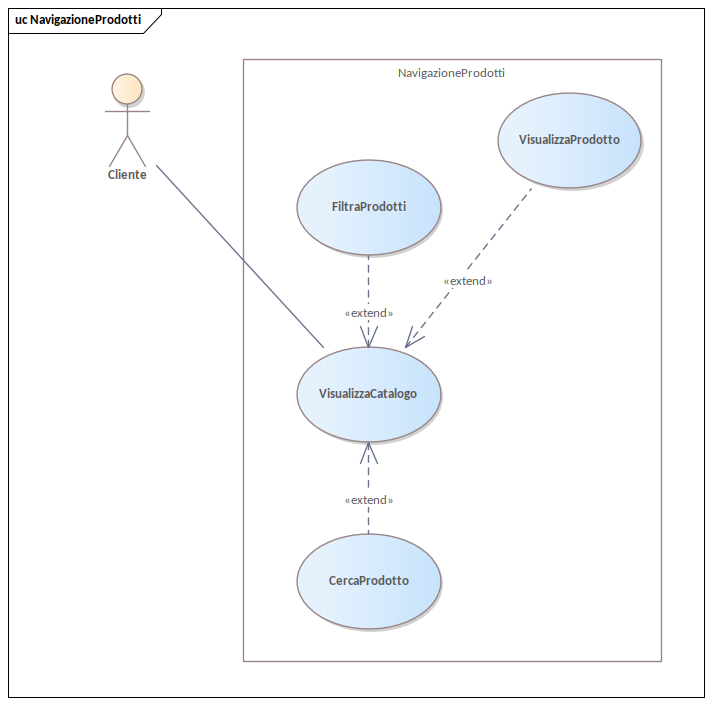
\includegraphics[width=\textwidth, height=20cm, keepaspectratio]{immagini/GestioneDeiRequisiti/NavigazioneProdotti.png}
\end{center}

\newpage
\paragraph{Caso d'uso: VisualizzaCatalogo}\mbox{}\\
\begin{center}
\begin{tabular}{ |p{12cm}| } 
    \hline
    \textbf{Caso d'uso: VisualizzaCatalogo} \\
    \hline
    \textbf{ID:} \theIDCasiDuso \stepcounter{IDCasiDuso} \\
    \hline
    \textbf{Breve Descrizione:} \\
    Il Cliente visualizza i prodotti del catalogo.\\
    \hline
    \textbf{Attori Primari:} \\
    Cliente \\
    \hline
    \textbf{Attori Secondari:} \\
    Nessuno \\
    \hline
    \textbf{Precondizioni:}
    \begin{enumerate}[nosep, left=0pt]
        \item Il Cliente visualizza la pagina home del sito.
    \end{enumerate}\\[-1em]
    \hline
    \textbf{Sequenza degli eventi principale:}
    \begin{enumerate}[nosep, left=0pt]
        \item Il caso d'uso inizia quando il Cliente seleziona "Visualizza tutti i prodotti" oppure "Visualizza i prodotti di una categoria".
        \item \textbf{If} il sistema trova almeno un prodotto
        \begin{enumerate}[nosep, left=0pt]
            \item[]\hspace*{-0.87cm} punto di estensione: Cerca prodotto
            \item[]\hspace*{-0.87cm} punto di estensione: Filtra prodotti
            \item \textbf{For each} prodotto trovato:
            \begin{enumerate}[nosep, left=0pt]
                \item Il sistema mostra al Cliente le seguenti informazioni del prodotto: nome, prezzo ed eventuale sconto, colori disponibili e immagine principale.
            \end{enumerate}
            \item[]\hspace*{-0.87cm} punto di estensione: Visualizza prodotto
        \end{enumerate}
        \item \textbf{Else} il sistema mostra al cliente che non sono stati trovati prodotti. 
    \end{enumerate} \\[-1em]
    \hline
    \textbf{Postcondizioni:} \\
    Nessuna \\
    \hline
    \textbf{Sequenza degli eventi alternativa:} \\
    Nessuna \\
    \hline
\end{tabular}
\end{center}


\newpage
\paragraph{Caso d'uso di estensione: CercaProdotto}\mbox{}\\
\begin{center}
\begin{tabular}{ |p{12cm}| } 
    \hline
    \textbf{Caso d'uso di estensione: CercaProdotto} \\
    \hline
    \textbf{ID:} \theIDCasiDuso \stepcounter{IDCasiDuso} \\
    \hline
    \textbf{Breve Descrizione:} \\
    Segmento 1: Il Cliente cerca il prodotto desiderato tramite ricerca testuale.\\
    \hline
    \textbf{Attori Primari:} \\
    Cliente \\
    \hline
    \textbf{Attori Secondari:} \\
    Nessuno \\
    \hline
    \textbf{Precondizioni del segmento 1:}
    \begin{enumerate}[nosep, left=0pt]
        \item Il Cliente visualizza il catalogo.
        \item Il Cliente seleziona "Cerca Prodotto".
    \end{enumerate}\\[-1em]
    \hline
    \textbf{Sequenza degli eventi del segmento 1:}
    \begin{enumerate}[nosep, left=0pt]
        \item Il Cliente inserisce le parole chiave del prodotto desiderato.
        \item Il sistema seleziona i prodotti che contengono almeno una parola di quelle inserite dal Cliente nelle seguenti informazioni del prodotto: nome,  descrizione, brand e colore. 
        \item \textbf{For each} prodotto selezionato:
        \begin{enumerate}[nosep, left=0pt]
            \item Il sistema assegna un valore da zero a uno al prodotto, calcolato tramite una formula matematica che permette di definirne il grado di affinità con la ricerca effettuata dall'utente.
        \end{enumerate}
        \item Il sistema mostra i prodotti selezionati, ordinati da quelli più affini a quelli meno affini.
    \end{enumerate} \\[-1em]
    \hline
    \textbf{Postcondizioni del segmento 1:} \\
    Nessuna \\
    \hline
\end{tabular}
\end{center}

\newpage
\paragraph{Caso d'uso di estensione: FiltraProdotti}\mbox{}\\
\begin{center}
\begin{tabular}{ |p{12cm}| } 
    \hline
    \textbf{Caso d'uso di estensione: FiltraProdotti} \\
    \hline
    \textbf{ID:} \theIDCasiDuso \stepcounter{IDCasiDuso} \\
    \hline
    \textbf{Breve Descrizione:} \\
    Segmento 1: Il Cliente filtra i prodotti per brand, colore e taglia.\\
    \hline
    \textbf{Attori Primari:} \\
    Cliente \\
    \hline
    \textbf{Attori Secondari:} \\
    Nessuno \\
    \hline
    \textbf{Precondizioni del segmento 1:}
    \begin{enumerate}[nosep, left=0pt]
        \item Il Cliente visualizza il catalogo.
        \item Il Cliente seleziona "Filtra Prodotti".
    \end{enumerate}\\[-1em]
    \hline
    \textbf{Sequenza degli eventi del segmento 1:}
    \begin{enumerate}[nosep, left=0pt]
        \item \textbf{If} Il cliente seleziona uno o più brand:
        \begin{enumerate}[nosep, left=0pt]
            \item \textbf{For each} brand selezionato:
            \begin{enumerate}[nosep, left=0pt]
                \item Il sistema seleziona i prodotti del brand selezionato
            \end{enumerate}
        \end{enumerate}
        \item \textbf{If} Il cliente seleziona uno o più colori:
        \begin{enumerate}[nosep, left=0pt]
            \item \textbf{For each} colore selezionato:
            \begin{enumerate}[nosep, left=0pt]
                \item Il sistema seleziona i prodotti che hanno una variante del colore selezionato.
            \end{enumerate}
        \end{enumerate}
        \item \textbf{If} Il cliente seleziona una o più taglie:
        \begin{enumerate}[nosep, left=0pt]
            \item \textbf{For each} taglia selezionata:
            \begin{enumerate}[nosep, left=0pt]
                \item Il sistema seleziona i prodotti che hanno una variante della taglia selezionata.
            \end{enumerate}
        \end{enumerate}
    \end{enumerate} \\[-1em]
    \hline
    \textbf{Postcondizioni del segmento 1:} \\
    Nessuna \\
    \hline
\end{tabular}
\end{center}

\newpage
\paragraph{Caso d'uso di estensione: VisualizzaProdotto}\mbox{}\\
\begin{center}
\begin{tabular}{ |p{12cm}| } 
    \hline
    \textbf{Caso d'uso di estensione: VisualizzaProdotto} \\
    \hline
    \textbf{ID:} \theIDCasiDuso \stepcounter{IDCasiDuso} \\
    \hline
    \textbf{Breve Descrizione:} \\
    Segmento 1: Il Cliente visualizza i dettagli di un prodotto \\
    \hline
    \textbf{Attori Primari:} \\
    Cliente \\
    \hline
    \textbf{Attori Secondari:} \\
    Nessuno \\
    \hline
    \textbf{Precondizioni del segmento 1:}
    \begin{enumerate}[nosep, left=0pt]
        \item Il Cliente visualizza il catalogo.
        \item Il Cliente seleziona l'opzione "Visualizza prodotto" da un prodotto del catalogo.
    \end{enumerate} \\
    \hline
    \textbf{Sequenza degli eventi del segmento 1:}
    \begin{enumerate}[nosep, left=0pt]
        \item Il sistema recupera i dettagli del prodotto selezionato.
        \item Il sistema mostra al cliente la pagina del prodotto con i seguenti dettagli: titolo, descrizione, prezzo ed eventuale sconto, immagini, ulteriori colori disponibili ed ulteriori taglie disponibili.
    \end{enumerate} \\
    \hline
    \textbf{Postcondizioni del segmento 1:}
    \begin{enumerate}[nosep, left=0pt]
        \item Il Cliente può aggiungere il prodotto al carrello.
    \end{enumerate} \\
    \hline
\end{tabular}
\end{center}


\newpage\paragraph{Diagramma GestioneCarrello}\mbox{}\\
\begin{center}
  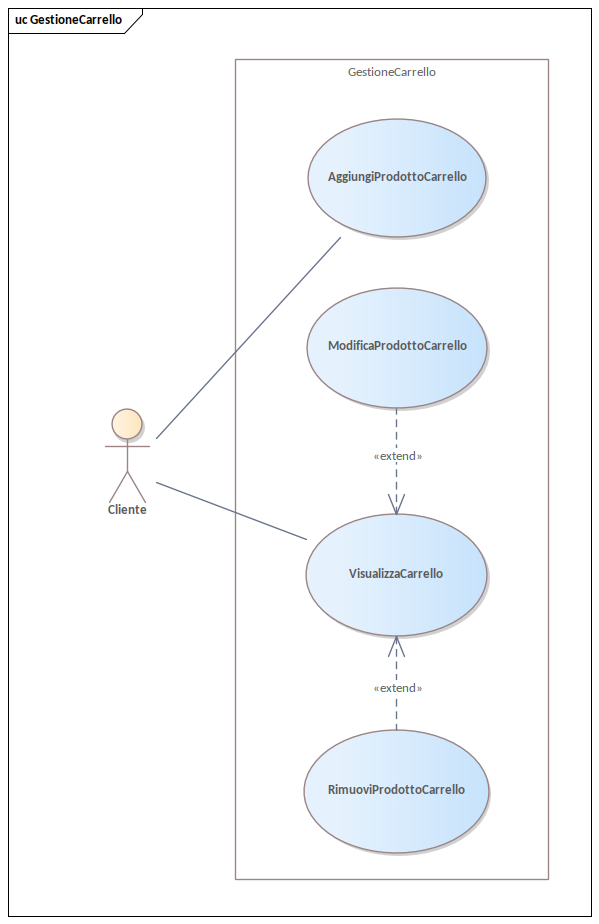
\includegraphics[width=\textwidth, height=20cm, keepaspectratio]{immagini/GestioneDeiRequisiti/GestioneCarrello.png}
\end{center}

\newpage
\paragraph{Caso d'uso: AggiungiProdottoCarrello}\mbox{}\\
\begin{center}
\begin{tabular}{ |p{12cm}| } 
    \hline
    \textbf{Caso d'uso: AggiungiProdottoCarrello} \\
    \hline
    \textbf{ID:} \theIDCasiDuso \stepcounter{IDCasiDuso} \\
    \hline
    \textbf{Breve Descrizione:} \\
    Un Cliente aggiunge un prodotto al carrello.  \\
    \hline
    \textbf{Attori Primari:} \\
    Cliente \\
    \hline
    \textbf{Attori Secondari:} \\
    Nessuno \\
    \hline
    \textbf{Precondizioni:}
    \begin{enumerate}[nosep, left=0pt]
    	\item Il Cliente visualizza la pagina del prodotto.
    	\item Il prodotto deve essere disponibile per l'acquisto.
            \item Il Cliente deve aver specificato la quantità desiderata del prodotto.
    \end{enumerate} \\
    \hline 
    \textbf{Sequenza degli eventi principale:}
    \begin{enumerate}[nosep, left=0pt]
        \item Il caso d'uso inizia quando il Cliente seleziona "Aggiungi al Carrello".
        \item Il sistema aggiunge il prodotto al carrello con la quantità specificata.
    \end{enumerate} \\
    \hline
    \textbf{Postcondizioni:} 
    \begin{enumerate}[nosep, left=0pt]
        \item Il prodotto è presente nel carrello con la quantità specificata dal Cliente. 
    \end{enumerate} \\
    \hline
    \textbf{Sequenza degli eventi alternativa:} \\
    Nessuna \\
    \hline
\end{tabular}
\end{center}

\newpage
\paragraph{Caso d'uso: VisualizzaCarrello}\mbox{}\\
\begin{center}
\begin{tabular}{ |p{12cm}| } 
    \hline
    \textbf{Caso d'uso: VisualizzaCarrello} \\
    \hline
    \textbf{ID:} \theIDCasiDuso \stepcounter{IDCasiDuso} \\
    \hline
    \textbf{Breve Descrizione:} \\
    Il Cliente visualizza il contenuto del carrello.  \\
    \hline
    \textbf{Attori Primari:} \\
    Cliente \\
    \hline
    \textbf{Attori Secondari:} \\
    Nessuno \\
    \hline
    \textbf{Precondizioni:} \\
    Nessuna \\
    \hline
    \textbf{Sequenza degli eventi principale:}
    \begin{enumerate}[nosep, left=0pt]
        \item Il caso d'uso inizia quando il Cliente seleziona "Visualizza Carrello".
        \item  Il sistema recupera i dettagli dei prodotti presenti nel carrello.
        \item \textbf{If} il sistema trova uno o più prodotti:
        \begin{enumerate}[nosep, left=0pt]
            \item \textbf{For} ogni prodotto trovato:
            \begin{enumerate}[nosep, left=0pt]
                \item Il sistema mostra le seguenti informazioni del prodotto: immagine principale, nome, quantità, colore, taglia e prezzo con eventuale sconto applicato.
                \item Il sistema mostra l'opzione "Rimuovi prodotto carrello" e "Modifica prodotto carrello".
                \item[]\hspace*{-1.2cm} punto di estensione: Modifica prodotto carrello
                \item[]\hspace*{-1.2cm} punto di estensione: Rimuovi prodotto carrello
                %l'opzione che definisce il prodotto come "attivo" (procedi all'ordine con questo prodotto) o "inattivo" (non procedere all'ordine con questo prodotto).
            \end{enumerate}
            \item Il sistema mostra il totale dell'ordine.
        \end{enumerate}
        \item \textbf{Else}
        \begin{enumerate}[nosep, left=0pt]
            \item Il sistema comunica al cliente che non sono stati trovati prodotti nel carrello.
        \end{enumerate}
    \end{enumerate} \\
    \hline
    \textbf{Postcondizioni:} 
    \begin{enumerate}[nosep, left=0pt]
        \item Il Cliente può procedere al checkout.
    \end{enumerate} \\
    \hline
    \textbf{Sequenza degli eventi alternativa:} \\
    Nessuna \\
    \hline
\end{tabular}
\end{center}

\newpage
\paragraph{Caso d'uso di estensione: ModificaProdottoCarrello}\mbox{}\\
\begin{center}
\begin{tabular}{ |p{12cm}| } 
    \hline
    \textbf{Caso d'uso di estensione: ModificaProdottoCarrello} \\
    \hline
    \textbf{ID:} \theIDCasiDuso \stepcounter{IDCasiDuso} \\
    \hline
    \textbf{Breve Descrizione:} \\
    Un Cliente modifica un prodotto nel carrello.  \\
    \hline
    \textbf{Attori Primari:} \\
    Cliente \\
    \hline
    \textbf{Attori Secondari:} \\
    Nessuno \\
    \hline
    \textbf{Precondizioni del segmento 1:}
    \begin{enumerate}[nosep, left=0pt]
    	\item Il Cliente visualizza la pagina del carrello.
        \item Il carrello non è vuoto.
        \item Il Cliente seleziona "Modifica prodotto carrello".
    \end{enumerate} \\
    \hline 
    \textbf{Sequenza degli eventi del segmento 1:}
    \begin{enumerate}[nosep, left=0pt]
        \item Il sistema richiede al Cliente di inserire le seguenti informazioni del prodotto del carrello: quantità, stato.
        \item \textbf{While} quantità minore di uno:
        \begin{enumerate}[nosep, left=0pt]
            \item Il Cliente inserisce le informazioni richieste.
        \end{enumerate}
	    \item Il sistema modifica il prodotto nel carrello.
    \end{enumerate} \\
    \hline
    \textbf{Postcondizioni del segmento 1:} 
    \begin{enumerate}[nosep, left=0pt]
        \item Le informazioni del prodotto nel carrello sono state aggiornate.
    \end{enumerate} \\
    \hline
\end{tabular}
\end{center}

\newpage
\paragraph{Caso d'uso di estensione: RimuoviProdottoCarrello}\mbox{}\\
\begin{center}
\begin{tabular}{ |p{12cm}| } 
    \hline
    \textbf{Caso d'uso di estensione: RimuoviProdottoCarrello} \\
    \hline
    \textbf{ID:} \theIDCasiDuso \stepcounter{IDCasiDuso} \\
    \hline
    \textbf{Breve Descrizione:} \\
    Il Cliente rimuove un prodotto dal carrello.  \\
    \hline
    \textbf{Attori Primari:} \\
    Cliente \\
    \hline
    \textbf{Attori Secondari:} \\
    Nessuno \\
    \hline
    \textbf{Precondizioni del segmento 1:}
    \begin{enumerate}[nosep, left=0pt]
    	\item Il Cliente visualizza la pagina del carrello. 
    	\item Il carrello non è vuoto. 
        \item Il Cliente seleziona l'opzione "Rimuovi prodotto carrello" su un prodotto presente nel carrello.
    \end{enumerate} \\
    \hline 
    \textbf{Sequenza degli eventi del segmento 1:}
    \begin{enumerate}[nosep, left=0pt]
        \item Il sistema rimuove il prodotto dal carrello.
    \end{enumerate} \\
    \hline
    \textbf{Postcondizioni del segmento 1:} 
    \begin{enumerate}[nosep, left=0pt] % La possibilità di avere questo layout per le postcondizioni è stata vista a pagina 62 del pdf Gestione dei Requisiti di Ursino
        \item Il prodotto non è più presente nel carrello. 
    \end{enumerate} \\
    \hline
\end{tabular}
\end{center}


\newpage\paragraph{Diagramma Gestione Ordine}\mbox{}\\
\begin{center}
  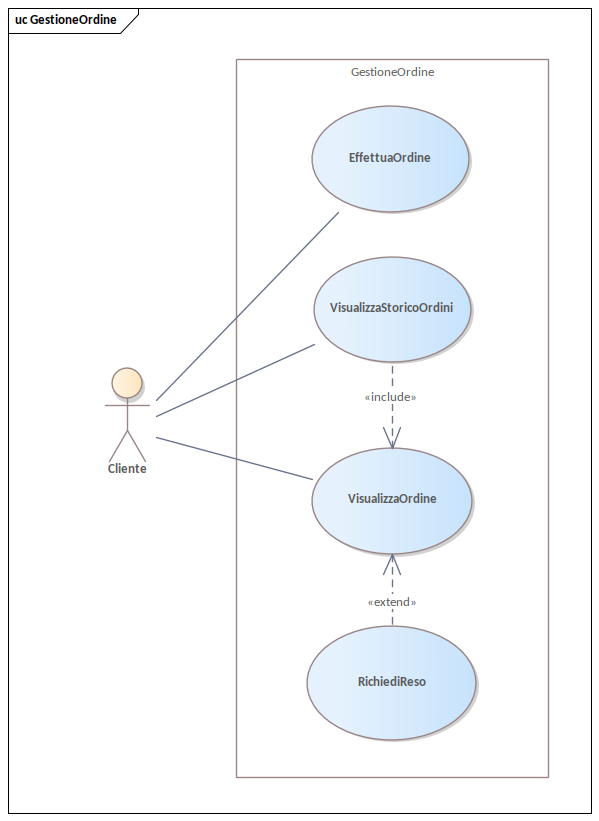
\includegraphics[width=\textwidth, height=20cm, keepaspectratio]{immagini/GestioneDeiRequisiti/GestioneOrdine.png}
\end{center}

\newpage
\paragraph{Caso d'uso: EffettuaOrdine}\mbox{}\\
\begin{center}
\begin{tabular}{ |p{12cm}| } 
    \hline
    \textbf{Caso d'uso: EffettuaOrdine} \\
    \hline
    \textbf{ID:} \theIDCasiDuso \stepcounter{IDCasiDuso} \\
    \hline
    \textbf{Breve Descrizione:} \\
    Il Cliente effettua un ordine.\\
    \hline
    \textbf{Attori Primari:} \\
    Cliente \\
    \hline
    \textbf{Attori Secondari:} \\
    Nessuno \\
    \hline
    \textbf{Precondizioni:} 
    \begin{enumerate}[nosep, left=0pt]
        \item Il Cliente deve aver effettuato l'accesso al proprio account.
    	\item Il Cliente visualizza il contenuto del carrello. 
    	\item Il carrello contiene almeno un prodotto con stato attivo.
    \end{enumerate} \\
    \hline 
    \textbf{Sequenza degli eventi principale:}
    \begin{enumerate}[nosep, left=0pt]
        \item Il caso d'uso inizia quando il Cliente seleziona l'opzione "Procedi all'acquisto".
        \item Il sistema mostra al Cliente la pagina di checkout con le seguenti informazioni: il prezzo totale e la lista dei prodotti da acquistare, corrispondenti a quelli con stato attivo nel carrello, con le relative informazioni.
        \item \textbf{While} le informazioni di spedizione non sono valide
        \begin{enumerate}[nosep, left=0pt]
            \item Il sistema chiede nuovamente al Cliente di inserire le informazioni di spedizione.
            \item Il sistema valida le informazioni di spedizione inserite dall'utente.
        \end{enumerate}
        \item Il Cliente seleziona la modalità di pagamento.
        \item Il Cliente seleziona "Effettua acquisto" per procedere al pagamento.
        \item \textbf{If} il pagamento va a buon fine:
        \begin{enumerate}[nosep, left=0pt]
            \item Il sistema crea l'ordine.
            \item Il sistema registra l'ordine effettuato.
        \end{enumerate}
        \item \textbf{Else}:
        \begin{enumerate}[nosep, left=0pt]
            \item Il sistema notifica al Cliente che il pagamento non è andato a buon fine.
            \item Il sistema mostra nuovamente al Cliente alla pagina di checkout.
        \end{enumerate}
    \end{enumerate} \\
    \hline
    \textbf{Postcondizioni:}
	\begin{enumerate}[nosep, left=0pt]
    	\item Il Cliente ha effettuato l'acquisto dei prodotti.
    \end{enumerate} \\
    \hline
    \textbf{Sequenza degli eventi alternativa:} \\
    Nessuna \\
    \hline
\end{tabular}
\end{center}

\newpage
\paragraph{Caso d'uso: VisualizzaOrdine}\mbox{}\\
\begin{center}
\begin{tabular}{ |p{12cm}| } 
    \hline
    \textbf{Caso d'uso: VisualizzaOrdine} \\
    \hline
    \textbf{ID:} \theIDCasiDuso \stepcounter{IDCasiDuso} \\
    \hline
    \textbf{Breve Descrizione:} \\
    Il Cliente visualizza i dettagli di un ordine effettuato. \\
    \hline
    \textbf{Attori Primari:} \\
    Cliente \\
    \hline
    \textbf{Attori Secondari:} \\
    Nessuno \\
    \hline
    \textbf{Precondizioni:} 
    \begin{enumerate}[nosep, left=0pt]
	    \item Il Cliente deve aver effettuato l'accesso al proprio account.
        \item Il Cliente visualizza la propria area personale.
	    \item L'ordine deve essere stato registrato nel sistema.
    \end{enumerate} \\
    \hline 
    \textbf{Sequenza degli eventi principale:}
    \begin{enumerate}[nosep, left=0pt]
        \item Il caso d'uso inizia quando il Cliente seleziona "Visualizza ordine" dalla lista degli ordini effettuati.
        \item Il sistema recupera i dettagli dell'ordine.
        \item \textbf{For} ogni prodotto ordinato:
        \begin{enumerate}[nosep, left=0pt]
            \item Il sistema mostra l'immagine principale del prodotto, il titolo, il prezzo e la quantità del prodotto.
        \end{enumerate}
        \item Il sistema mostra l'indirizzo di spedizione specificato, il metodo di pagamento utilizzato e la data di effettuazione dell'ordine.
    \end{enumerate} \\
    \hline
    \textbf{Postcondizioni:} \\
	Nessuna \\
    \hline
    \textbf{Sequenza degli eventi alternativa:} \\
    Nessuna \\
    \hline
\end{tabular}
\end{center}

\newpage
\paragraph{Caso d'uso: VisualizzaStoricoOrdini}\mbox{}\\
\begin{center}
\begin{tabular}{ |p{12cm}| } 
    \hline
    \textbf{Caso d'uso: VisualizzaStoricoOrdini} \\
    \hline
    \textbf{ID:} \theIDCasiDuso \stepcounter{IDCasiDuso} \\
    \hline
    \textbf{Breve Descrizione:} \\
    Il Cliente visualizza i dettagli di tutti gli ordini effettuati. \\
    \hline
    \textbf{Attori Primari:} \\
    Cliente \\
    \hline
    \textbf{Attori Secondari:} \\
    Nessuno \\
    \hline
    \textbf{Precondizioni:} 
    \begin{enumerate}[nosep, left=0pt]
	    \item Il Cliente deve aver effettuato l'accesso al proprio account.
        \item Il Cliente visualizza la propria area personale.
    \end{enumerate} \\
    \hline 
    \textbf{Sequenza degli eventi principale:}
    \begin{enumerate}[nosep, left=0pt]
        \item Il caso d'uso inizia quando il Cliente seleziona "Visualizza storico ordini" dalla propria area personale.
        \item Il sistema recupera i dettagli degli ordini.
        \item \textbf{If} il Cliente ha almeno un ordine registrato nel sistema 
        \begin{enumerate}[nosep, left=0pt]
        \item \textbf{For} ogni ordine del cliente:
        \begin{enumerate}[nosep, left=0pt]
            \item Include (VisualizzaOrdine)
        \end{enumerate}
        \end{enumerate}
        \item \textbf{Else}
        \begin{enumerate}[nosep, left=0pt]
            \item Il sistema avvisa il cliente che non ha nessun ordine registrato nel sistema
        \end{enumerate}
    \end{enumerate} \\
    \hline
    \textbf{Postcondizioni:} \\
	Nessuna \\
    \hline
    \textbf{Sequenza degli eventi alternativa:} \\
    Nessuna \\
    \hline
\end{tabular}
\end{center}

\newpage
\paragraph{Caso d'uso di estensione: RichiediReso}\mbox{}\\
\begin{center}
\begin{tabular}{ |p{12cm}| } 
    \hline
    \textbf{Caso d'uso di estensione: RichiediReso} \\
    \hline
    \textbf{ID:} \theIDCasiDuso \stepcounter{IDCasiDuso} \\
    \hline
    \textbf{Breve Descrizione:} \\
    Segmento 1: Il Cliente richiede il reso di un prodotto ordinato. \\
    \hline
    \textbf{Attori Primari:} \\
    Cliente \\
    \hline
    \textbf{Attori Secondari:} \\
    Nessuno \\
    \hline
    \textbf{Precondizioni del segmento 1:} 
    \begin{enumerate}[nosep, left=0pt]
	    \item Il Cliente deve aver eseguito l'accesso al proprio account.
	    \item Il Cliente deve aver selezionato un ordine effettuato in precedenza.
        \item Il Cliente seleziona l'opzione "Richiedi Reso" di un prodotto presente nella lista dei prodotti ordinati.
    \end{enumerate} \\
    \hline 
    \textbf{Sequenza degli eventi del segmento 1:}
    \begin{enumerate}[nosep, left=0pt]
        \item Il sistema chiede al Cliente di inserire le informazioni del reso: motivazione e descrizione. 
        \item Il Cliente conferma la richiesta di reso.
    \end{enumerate} \\
    \hline
    \textbf{Postcondizioni del segmento 1:} 
	\begin{enumerate}[nosep, left=0pt]
        \item Il reso è stato registrato nel sistema.
	\end{enumerate} \\
    \hline
\end{tabular}
\end{center}


\newpage\paragraph{Diagramma Gestione Recensione}\mbox{}\\
\begin{center}
  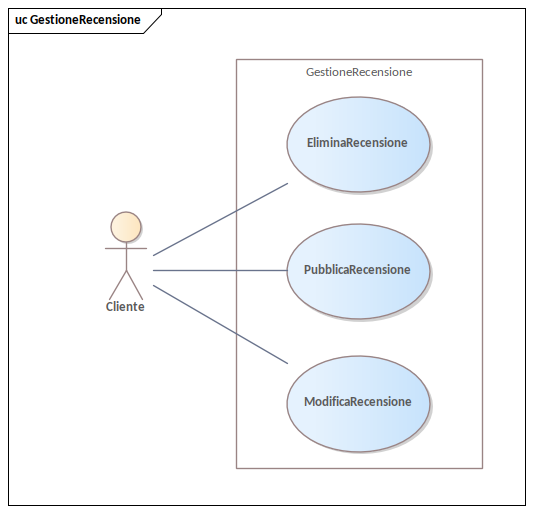
\includegraphics[width=\textwidth, height=20cm, keepaspectratio]{immagini/GestioneDeiRequisiti/GestioneRecensione.png}
\end{center}

\newpage
\paragraph{Caso d'uso: PubblicaRecensione}\mbox{}\\
\begin{center}
\begin{tabular}{ |p{12cm}| } 
    \hline
    \textbf{Caso d'uso: PubblicaRecensione} \\
    \hline
    \textbf{ID:} \theIDCasiDuso \stepcounter{IDCasiDuso} \\
    \hline
    \textbf{Breve Descrizione:} \\
    Il Cliente pubblica una recensione per un prodotto che ha acquistato.\\
    \hline
    \textbf{Attori Primari:} \\
    Cliente \\
    \hline
    \textbf{Attori Secondari:} \\
    Nessuno \\
    \hline
    \textbf{Precondizioni:} 
    \begin{enumerate}[nosep, left=0pt]
    \item Il Cliente ha effettuato l'accesso al proprio account.
    \item Il Cliente ha ordinato il prodotto di cui vuole pubblicare una recensione.
    \item Il Cliente non ha già pubblicato una recensione del prodotto.
	\item Il Cliente visualizza la pagina del prodotto di cui vuole pubblicare una recensione. 
    \end{enumerate} \\
    \hline 
    \textbf{Sequenza degli eventi principale:}
    \begin{enumerate}[nosep, left=0pt]
        \item Il caso d'uso inizia quando il Cliente seleziona l'opzione "Pubblica una recensione".
	    \item Il sistema richiede al Cliente di inserire le seguenti informazioni della recensione: titolo, descrizione e voto.
        \item Il Cliente inserisce le informazioni della recensione richieste.
	    \item Il sistema aggiunge la recensione alla pagina prodotto.
    \end{enumerate} \\
    \hline
    \textbf{Postcondizioni:}
	\begin{enumerate}[nosep, left=0pt]
    	\item Il Cliente ha pubblicato una recensione del prodotto.
    \end{enumerate} \\
    \hline
    \textbf{Sequenza degli eventi alternativa:} \\
    Nessuna \\
    \hline
\end{tabular}
\end{center}

\newpage
\paragraph{Caso d'uso: ModificaRecensione}\mbox{}\\
\begin{center}
\begin{tabular}{ |p{12cm}| } 
    \hline
    \textbf{Caso d'uso: ModificaRecensione} \\
    \hline
    \textbf{ID:} \theIDCasiDuso \stepcounter{IDCasiDuso} \\
    \hline
    \textbf{Breve Descrizione:} \\
    Il Cliente modifica la recensione di un prodotto che ha precedentemente pubblicato.\\
    \hline
    \textbf{Attori Primari:} \\
    Cliente \\
    \hline
    \textbf{Attori Secondari:} \\
    Nessuno \\
    \hline
    \textbf{Precondizioni:} 
    \begin{enumerate}[nosep, left=0pt]
	    \item Il Cliente ha effettuato l'accesso al proprio account.
        \item Il Cliente ha pubblicato una recensione del prodotto.
    	\item Il Cliente visualizza la pagina del prodotto di cui ha pubblicato una recensione. 
    \end{enumerate} \\
    \hline 
    \textbf{Sequenza degli eventi principale:}
    \begin{enumerate}[nosep, left=0pt]
        \item Il caso d'uso inizia quando il Cliente seleziona "Modifica Recensione".
	    \item Il sistema richiede al Cliente di inserire le seguenti informazioni della recensione: titolo, descrizione e voto.
        \item Il Cliente inserisce le informazioni della recensione richieste.
	    \item Il sistema modifica la recensione del Cliente.
    \end{enumerate} \\
    \hline
    \textbf{Postcondizioni:} \\
	\begin{enumerate}[nosep, left=0pt]
    	\item I dettagli della recensione sono stati aggiornati.
    \end{enumerate} \\
    \hline
    \textbf{Sequenza degli eventi alternativa:} \\
    Nessuna \\
    \hline
\end{tabular}
\end{center}

\newpage
\paragraph{Caso d'uso: EliminaRecensione}\mbox{}\\
\begin{center}
\begin{tabular}{ |p{12cm}| } 
    \hline
    \textbf{Caso d'uso: EliminaRecensione} \\
    \hline
    \textbf{ID:} \theIDCasiDuso \stepcounter{IDCasiDuso} \\
    \hline
    \textbf{Breve Descrizione:} \\
    Il Cliente elimina la recensione di un prodotto che ha precedentemente pubblicato.\\
    \hline
    \textbf{Attori Primari:} \\
    Cliente \\
    \hline
    \textbf{Attori Secondari:} \\
    Nessuno \\
    \hline
    \textbf{Precondizioni:} 
    \begin{enumerate}[nosep, left=0pt]
	    \item Il Cliente ha effettuato l'accesso al proprio account.
        \item Il Cliente ha pubblicato una recensione del prodotto.
    	\item Il Cliente visualizza la pagina del prodotto di cui ha pubblicato una recensione. 
    \end{enumerate} \\
    \hline 
    \textbf{Sequenza degli eventi principale:}
    \begin{enumerate}[nosep, left=0pt]
        \item Il caso d'uso inizia quando il Cliente seleziona "Elimina recensione".
        \item Il sistema rimuove la recensione dalla pagina prodotto.
    \end{enumerate} \\
    \hline
    \textbf{Postcondizioni:} \\
	\begin{enumerate}[nosep, left=0pt]
    	\item La recensione del prodotto è stata eliminata.
    \end{enumerate} \\
    \hline
    \textbf{Sequenza degli eventi alternativa:} \\
    Nessuna \\
    \hline
\end{tabular}
\end{center}


\newpage\section{Matrice di Mapping}
\label{sec:MatriceDiMapping}
\begin{center}
  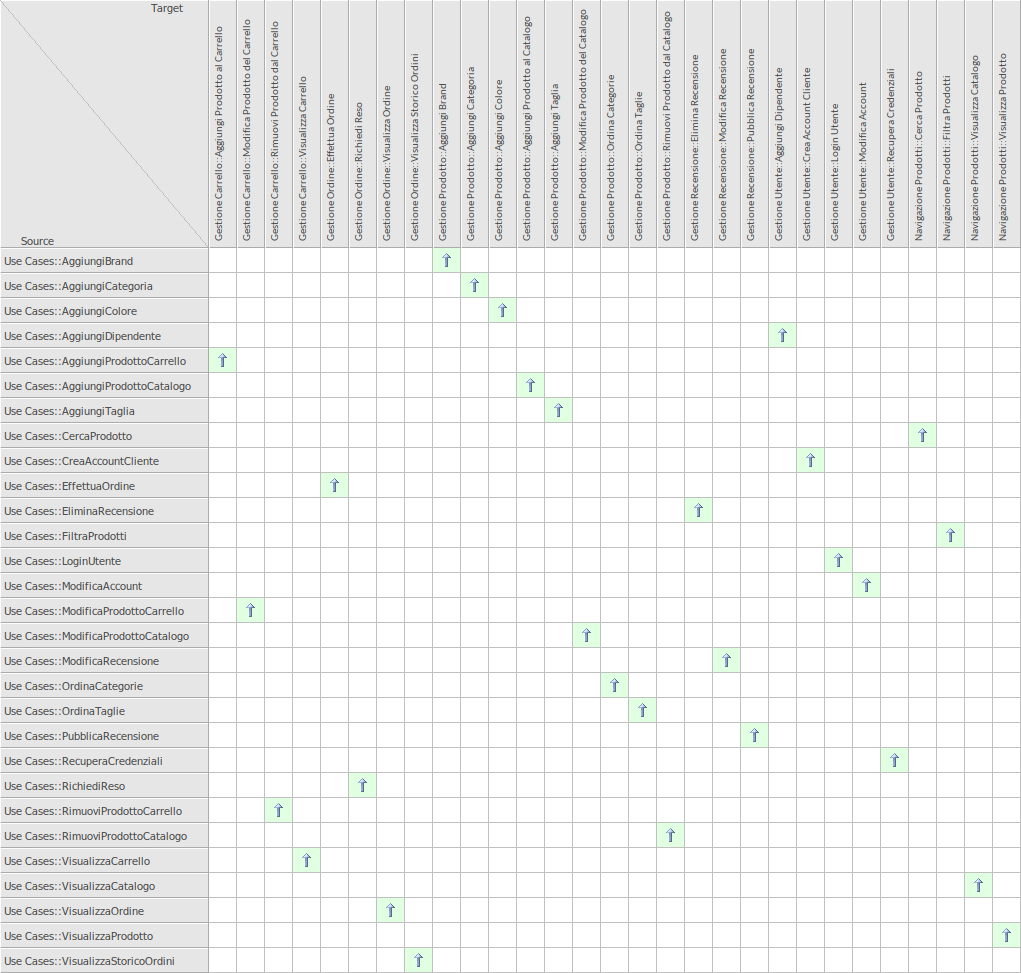
\includegraphics[width=\textwidth, height=20cm, keepaspectratio]{immagini/GestioneDeiRequisiti/MatriceDiMapping.png}
\end{center}